\documentclass{report}
\usepackage{multirow}
\usepackage[table]{xcolor}
\usepackage{geometry}
\usepackage{hhline}
\usepackage{graphicx}
\usepackage{hyperref}
\graphicspath{ {C:/Users/dimri/Desktop/CD/img/}	}
 \geometry{
 a4paper,
 total={170mm,257mm},
 left=12mm,
 top=20mm,
 }
\begin{document}

\begin{titlepage}
   \begin{center}
       \vspace*{5cm}
		\Huge
       \textbf{VHDL SPECIFICATION}

       \vspace{0.5cm}
       \LARGE
        Circuit Design (WS2021/22)\\
		Prof. Dr. -Ing Andreas Siggelkow\\
            
       \vspace{1cm}

       \textbf{Engli Shehu \& Amir Reza Edalati} 
       
       \vspace{2cm}
       
       
\includegraphics[width=0.4\textwidth]{logo.png}
       
       \vfill
            
       \vspace{0.8cm}
            
       Hochschule Ravensburg-Weingarten\\
       Germany\\
       09.11.2021\\
            
   \end{center}
\end{titlepage}
\newpage

\large
\tableofcontents

\newpage

\chapter{History - Change Log}

\begin{table}[ht!]
\begin{center}
\large
\newcolumntype{P}[1]{>{\centering\arraybackslash}p{#1}}
\renewcommand{\arraystretch}{1.7}
\begin{tabular}{ |P{3cm}|P{3cm}|P{10cm}|}
 \hline
 \rowcolor{gray!50} \textbf{Version} & \textbf{Date} & \textbf{Description}   \\
 \hline
 V 0.1 & 26.10.2021 & Requirements Table  \\
 \hline
 V 0.2 & 09.11.2021 & Spefication added  \\
 \hline
  V 0.3 & 08.12.2021 & Timer and counter entities  \\
 \hline
  V 0.4 & 13.12.2021 & Full top level and running simulation without uart\\
 \hline
  V 0.5 & 18.12.2021 & Complete uart and synthesis   \\
 \hline
  V 0.6 & 06.01.2022 & Errors are fixed  \\
 \hline
  V 0.7 & 15.01.2022 & Top level changed  \\
 \hline
  V 1.0 & 17.01.2022 & Final specification  \\
 \hline
\end{tabular}
\end{center}
\end{table}

\vfill
\begin{table}
 \begin{center}
 \Large
\newcolumntype{P}[1]{>{\centering\arraybackslash}p{#1}}
\renewcommand{\arraystretch}{1.7}
\begin{tabular}{ P{6cm}P{6cm}}
\hline
 \hline
 \cellcolor{gray!50} \textbf{Current Version:} & V 1.0\\
 \cellcolor{gray!50} \textbf{Description:} & Final Specification\\
 \hline
 \hline
\end{tabular}
\end{center}
\end{table}
\vspace{3cm}
\newpage

\chapter{Description}
\Large
This is an application which aims to control the brewing time of a teabag. The system uses a single sensor to detect when a Tea Bag is dropped in, so this solution is only feasable on the condition that only one tabag is being brewed at a time. The brewing time is adjustable between 2:00-5:00 min. After the brewing time is done the system will ring an alarm to notify procedure finished and than the time is recorded. After this the system is rearmed again. The Data is saved on a PC to be accessed later. 
\vspace{1.5cm}
\begin{figure}[htbp]
\centerline{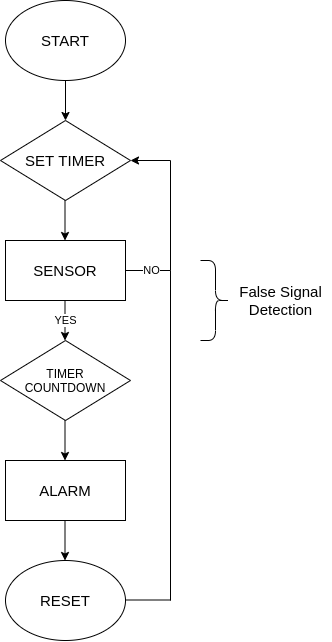
\includegraphics[width=7cm, height=12cm]{flowchart}}
\caption{Flowchart.}
\label{fig}
\end{figure}
\newpage

\chapter{Requirements Table}
\begin{table}[ht!]
 \begin{center}
\newcolumntype{P}[1]{>{\centering\arraybackslash}p{#1}}
\renewcommand{\arraystretch}{1.4}
\begin{tabular}{ |P{0,7cm}|P{2,5cm}|P{2cm}|P{2,8cm} |P{8cm}|}
 \hline
 \rowcolor{blue!25}\large ID&\large Name & \large Importance & \large Test & \large Description\\
 \hline
\hline
 \rowcolor{blue!25}\multicolumn{5}{|c|}{\large \textbf{General}}\\
 \hline
 \cellcolor{gray!30}G1,1  &  \cellcolor{gray!30}Time & High & VHDL Testbench & Time of brewing. \\ 
 \hline
 \cellcolor{gray!30}G1,2  &  \cellcolor{gray!30}Start & High & VHDL Testbench & Remarks when the Tea Bag is droppped in. \\
 \hline
\cellcolor{gray!30}G1,3  &  \cellcolor{gray!30}Stop & High & VHDL Testbench & Notifies when the brewing should stop. \\
 \hline
\hline
 \rowcolor{blue!25}\multicolumn{5}{|c|}{\large \textbf{Interface}}\\
 \hline
\cellcolor{gray!30}I2,1  &  \cellcolor{gray!30}Sensor & High & VHDL Testbench & Senses when the Tea Bag is dropped in.  \\
 \hline
\cellcolor{gray!30}I2,2  &  \cellcolor{gray!30}Alarm & High & VHDL Testbench & Activated when the brewing should Stop.  \\
 \hline
\cellcolor{gray!30}I2,3  &  \cellcolor{gray!30}GPS & High & VHDL Testbench & Sends the time via the NMEA Dataset. \\
 \hline
\cellcolor{gray!30}I2,4  &  \cellcolor{gray!30}Local Key & High & VHDL Testbench & Sends the time localy. \\
 \hline
\cellcolor{gray!30}I2,5  &  \cellcolor{gray!30}ASCII-receiver-interface & High & VHDL Testbench & Expects a time in Seconds in ASCII format.  \\
 \hline
 \hline
 \rowcolor{blue!25}\multicolumn{5}{|c|}{\large \textbf{UART}}\\
 \hline
\cellcolor{gray!30}U3,1  &  \cellcolor{gray!30}9K6 & High & VHDL Testbench & The speed of the serial transmission shouuld be set to 9600 baud.  \\
 \hline
\cellcolor{gray!30}U3,2  &  \cellcolor{gray!30}8N2 & High & VHDL Testbench & The data width of the serial transmission should be set to 8 bit.  \\
 \hline
\cellcolor{gray!30}U3,3  &  \cellcolor{gray!30}8N2 & High & VHDL Testbench & The serial transmission should not be checked with a parity bit.  \\
 \hline
\cellcolor{gray!30}U3,4  &  \cellcolor{gray!30}8N2 & High & VHDL Testbench & The serial transmission should have twos stop bits.  \\
 \hline
\cellcolor{gray!30}U3,5  &  \cellcolor{gray!30}UART Time & High & VHDL Testbench & The time stamp the event should be delivered to a PC.  \\
 \hline
\cellcolor{gray!30}U3,6  &  \cellcolor{gray!30}UART Start & High & VHDL Testbench & The start of the event should be delivered to a PC.  \\
 \hline
\cellcolor{gray!30}U3,7  &  \cellcolor{gray!30}UART Stop & High & VHDL Testbench & Ending of the event should be delivered to a PC.  \\
 \hline
\cellcolor{gray!30}U3,8  &  \cellcolor{gray!30}Working Data & High & VHDL Testbench & Working Data should be stored in 32-bit registers. \\
 \hline
\cellcolor{gray!30}U3,9  &  \cellcolor{gray!30}UART-RX & High & VHDL Testbench & 32-bit Registers should be loadable by UART-RX\\
 \hline
\cellcolor{gray!30}U3,10  &  \cellcolor{gray!30}UART-TX & High & VHDL Testbench & 32-bit Registers should be readable by UART-TX\\
 \hline
\cellcolor{gray!30}U3,11 &  \cellcolor{gray!30}Register Accessibility & High & VHDL Testbench & 32-bit Registers should be adressable\\
 \hline
 \hline
 \rowcolor{blue!25}\multicolumn{5}{|c|}{\large \textbf{PC}}\\
\hline
\cellcolor{gray!30}P4,1 &  \cellcolor{gray!30}PC Language & High & PC & The Programming Language is C++\\
 \hline

\end{tabular}
\end{center}
\end{table}
\newpage

\chapter{Top Level View}
\section{Block Diagram}
\begin{figure}[htbp]
{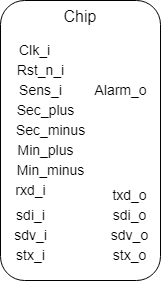
\includegraphics[width=5cm, height=8cm]{chip}}
\hspace{3cm}
{\includegraphics[width=10cm, height=9cm]{max1000}}
\caption{Top View.}
\label{fig}
\end{figure}
\begin{figure}[htbp]
\centerline{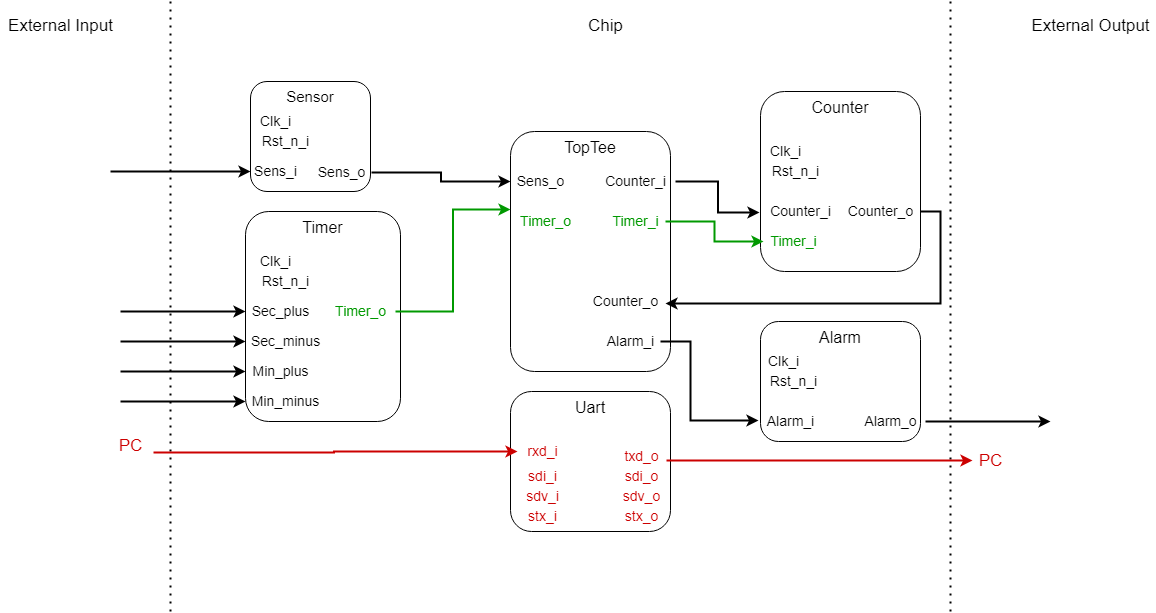
\includegraphics[width=18cm, height=9cm]{top_level.png}}
\caption{Top Level Block Diagram.}
\label{fig}
\vspace{2cm}
\centerline{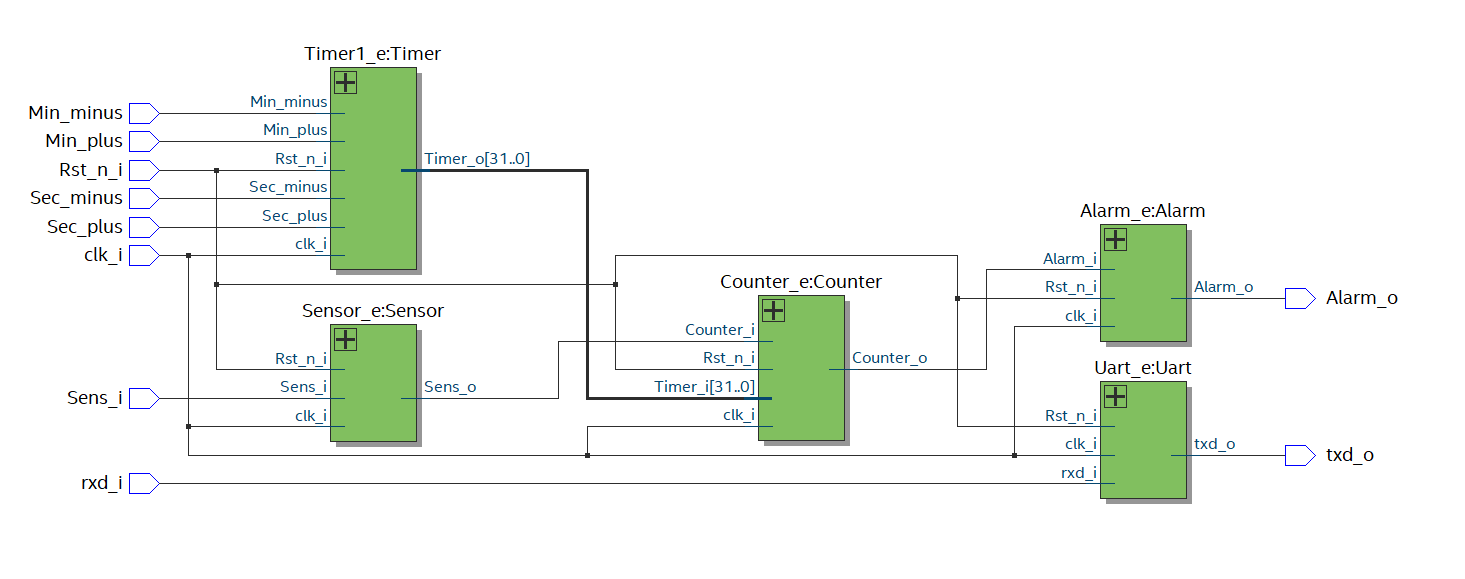
\includegraphics[width=18cm, height=9cm]{top_level_rtl.png}}
\caption{Top Level Block Diagram Rtl.}
\label{fig}
\end{figure}
\newpage

\section{Description}
\large
The Top Level consists of the following entities: \\
- Timer\_e \\
  In the timer entity we take external inputs from the user for which we set the time that the tea has to boil. Then we send the time to the counter. \\
- Counter\_e \\
  In the counter we receive two inputs, one from the timer and the other from sensor. Then we count down the time and at the end we output the signal.\\
- Sensor\_e \\
  In the sensor we receive an external output signal, debounce it and then output it. The sensor is triggered when the tea bag is dropped.\\
- Alarm\_e \\
  In the alarm we output a signal for three seconds.\\
- Uart\_e\\
  In the Uart we receive and transmit data with the local PC.\\
   

\vspace{2cm}

\section{Top level signal list}
\begin{table}[ht!]
\begin{center}
\large
\newcolumntype{P}[1]{>{\centering\arraybackslash}p{#1}}
\renewcommand{\arraystretch}{1.5}
\begin{tabular}{ |P{2cm}|P{2cm}|P{2cm}|P{8cm}|}
 \hline
 \rowcolor{gray!50} \textbf{Pin} & \textbf{Direction } & \textbf{Width}  & \textbf{Description} \\
 \hline
 clk\_i & IN & 1 & 12MHz\\
 \hline
 Rst\_n\_i & IN & 1 & Reset, Active Low \\
 \hline
 Sec\_plus & IN & 1 & Increment one second \\
 \hline
 Sec\_minus & IN & 1 & Decrement one second \\
 \hline
 Min\_plus & IN & 1 & Increment sixty seconds \\
 \hline
 Min\_minus & IN & 1 & Decrement sixty seconds \\
 \hline
 Sens\_i & IN & 1 & Input from external sensor \\
 \hline
 Alarm\_o & OUT & 1 & Output to external source \\
 \hline
 rxd\_i & IN & 1 & Data input from Uart \\
 \hline
 txd\_o & OUT & 1 & Data output from Uart \\
 \hline
 Timer\_o & Signal & 32 & Output time from timer \\
 \hline
 Timer\_i & Signal & 32 & Input time to counter \\
 \hline
Counter\_i & Signal & 1 & Start signal for counter \\
 \hline
Counter\_o & Signal & 1 & Output signal from counter \\
 \hline
Alarm\_i & Signal & 1 & Start signal for alarm \\
 \hline
\end{tabular}
\end{center}
\end{table}
\chapter{System Design}
\section{Sensor}
\begin{figure}[htbp]
	\centerline{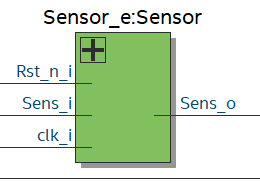
\includegraphics[width=6cm, height=6cm]{sensor.png}}
	\caption{Sensor Top Level.}
	\label{fig}
\end{figure}
\begin{table}[ht!]
	\begin{center}
		\large
		\newcolumntype{P}[1]{>{\centering\arraybackslash}p{#1}}
		\renewcommand{\arraystretch}{1.5}
		\begin{tabular}{ |P{2cm}|P{2cm}|P{2cm}|P{8cm}|}
			\hline
			\rowcolor{gray!50} \textbf{Pin} & \textbf{Direction } & \textbf{Width}  & \textbf{Description} \\
			\hline
			clk\_i & IN & 1 & 12MHz\\
			\hline
			Rst\_n\_i & IN & 1 & Reset, Active Low \\
			\hline
			Sens\_i  & IN & 1 & Input from external sensor  \\
			\hline
			Sens\_o  & OUT & 1 & Output after debounce \\
			\hline
			debouncer\_1  & Signal & 1 &   \\
			\hline
			debouncer\_2  & Signal & 1 &   \\
			\hline
		\end{tabular}
	\end{center}
\end{table}
\LARGE
DESCRITPION \\
\\
\Large
 In our system we operate the sensor using a push button. At first the signal is debounced in order to make sure that the system is not triggered by noise. After this the sensor gives an output when the button is released. This is done in order t prevent the sensor from triggering repeatedly.  

\vspace{1.5cm}
\newpage
\section{Timer}
\vspace{1cm}
\begin{figure}[htbp]
	\centerline{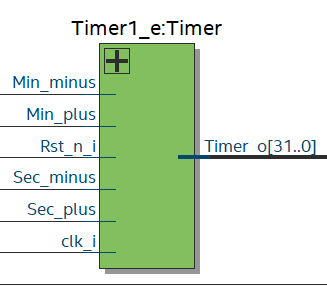
\includegraphics[width=6cm, height=6cm]{timer.png}}
	\caption{Timer Top Level.}
	\label{fig}
\end{figure}
\vspace{1cm}
\begin{table}[ht!]
	\begin{center}
		\large
		\newcolumntype{P}[1]{>{\centering\arraybackslash}p{#1}}
		\renewcommand{\arraystretch}{1.5}
		\begin{tabular}{ |P{2cm}|P{2cm}|P{2cm}|P{8cm}|}
			\hline
			\rowcolor{gray!50} \textbf{Pin} & \textbf{Direction } & \textbf{Width}  & \textbf{Description} \\
			\hline
			clk\_i & IN & 1 & 12MHz\\
			\hline
			Rst\_n\_i & IN & 1 & Reset, Active Low \\
			\hline
			Sec\_plus & IN & 1 & Increment one second \\
			\hline
			Sec\_minus & IN & 1 & Decrement one second \\
			\hline
			Min\_plus & IN & 1 & Increment sixty seconds \\
			\hline
			Min\_minus & IN & 1 & Decrement sixty seconds \\
			\hline
			Timer\_o & OUT & 32 & Register for sending time \\
			\hline
			timer & Signal & 32 &  \\   
			\hline
			debouncer\_1 & Signal & 1 &  \\   
			\hline
			debouncer\_2 & Signal & 1 &  \\   
			\hline
			timer\_state & FSM & 5 states & \\
			\hline 
			state & signal & 1 & \\
			\hline  
		\end{tabular}
	\end{center}
\end{table}
\LARGE
DESCRITPION \\
\\
\Large
In our system we set the time using four input signals that the user drives. Afterwards the time is saved to a register and then outputed inside the system for counting. All the input signals are arranged via a FSM and all of them are debounced. The system is designed so that if a tea is already boiling the timer ca not be changed.  
\vspace{1.5cm}
\newpage
\section{Counter}
\vspace{1cm}
\begin{figure}[htbp]
	\centerline{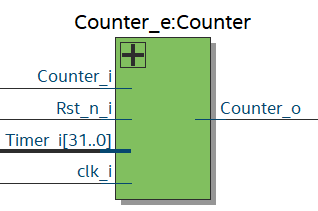
\includegraphics[width=6cm, height=6cm]{counter.png}}
	\caption{Counter Top Level.}
	\label{fig}
\end{figure}
\vspace{1cm}
\begin{table}[ht!]
	\begin{center}
		\large
		\newcolumntype{P}[1]{>{\centering\arraybackslash}p{#1}}
		\renewcommand{\arraystretch}{1.5}
		\begin{tabular}{ |P{2cm}|P{2cm}|P{2cm}|P{8cm}|}
			\hline
			\rowcolor{gray!50} \textbf{Pin} & \textbf{Direction } & \textbf{Width}  & \textbf{Description} \\
			\hline
			clk\_i & IN & 1 & 12MHz\\
			\hline
			Rst\_n\_i & IN & 1 & Reset, Active Low \\
			\hline
			Timer\_i & IN & 32 & Timer register \\
			\hline
			Counter\_i & IN & 1 & Signal to start counting \\
			\hline
			Counter\_o & OUT & 1 & Output signal when finished counting \\
			\hline
			Ticks & Signal & 32 &  \\
			\hline
			Seconds & Signal & 32 &  \\
			\hline
		     Counter\_input & Signal & 32 &  \\   
			\hline
			 Counter\_state & Signal & 1 &  \\   
			\hline 
		\end{tabular}
	\end{center}
\end{table}
\LARGE
DESCRITPION \\
\\
\Large
The counter entity requires two inputs. First input is taken from the debounced sensor and starts the countdown of the time. The second input is the 32 bit time register which should not be zero for the counter to starts its process. In the counter we count every rising edge and save it to a register until ewe have one second. Then we save its to another register and count it until our value matches the timer input. When the values are equal the counter sends the output signal high to the alarm entity. 
\vspace{1.5cm}
\newpage
\section{Alarm}
\vspace{1cm}
\begin{figure}[htbp]
	\centerline{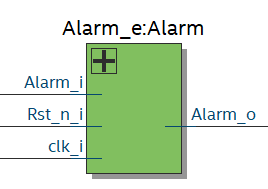
\includegraphics[width=6cm, height=6cm]{alarm.png}}
	\caption{Alarm Top Level.}
	\label{fig}
\end{figure}
\vspace{1cm}
\begin{table}[ht!]
	\begin{center}
		\large
		\newcolumntype{P}[1]{>{\centering\arraybackslash}p{#1}}
		\renewcommand{\arraystretch}{1.5}
		\begin{tabular}{ |P{2cm}|P{2cm}|P{2cm}|P{8cm}|}
			\hline
			\rowcolor{gray!50} \textbf{Pin} & \textbf{Direction } & \textbf{Width}  & \textbf{Description} \\
			\hline
			clk\_i & IN & 1 & 12MHz\\
			\hline
			Rst\_n\_i & IN & 1 & Reset, Active Low \\
			\hline
			Timer\_i & IN & 32 & Timer register \\
			\hline
			Alarm\_i & IN & 1 & Input signal to start the alarm process \\
			\hline
			Alarm\_o & OUT & 1 & Output signal to alarm module \\
			\hline
			ticks & Signal & 32 &  \\
			\hline
			state & Signal & 1 &  \\
			\hline
		\end{tabular}
	\end{center}
\end{table}
\LARGE
DESCRITPION \\
\\
\Large
The alarm entity receives an input signal to start counting for three seconds. While it is counting, it outputs a high signal which is wired to the external alarm module. The same procedure as in the counter is used to countdown three seconds. When the countdown is finished, the output signal goes back to low and the alarm is in a ready state again.
\vspace{1.5cm}
\newpage
\section{Uart}
\vspace{1cm}
\begin{figure}[htbp]
	\centerline{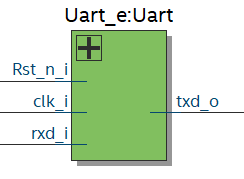
\includegraphics[width=6cm, height=6cm]{uart.png}}
	\caption{Uart Top Level.}
	\label{fig}
\end{figure}
\vspace{1cm}
\begin{table}[ht!]
	\begin{center}
		\large
		\newcolumntype{P}[1]{>{\centering\arraybackslash}p{#1}}
		\renewcommand{\arraystretch}{1.5}
		\begin{tabular}{ |P{2cm}|P{2cm}|P{2cm}|P{8cm}|}
			\hline
			\rowcolor{gray!50} \textbf{Pin} & \textbf{Direction } & \textbf{Width}  & \textbf{Description} \\
			\hline
			clk\_i & IN & 1 & 12MHz\\
			\hline
			Rst\_n\_i & IN & 1 & Reset, Active Low \\
			\hline
			rxd\_i & IN & 1 & received data signal\\
			\hline\
			txd\_o & OUT & 1 & transmitted data signal\\
			\hline
			state & FSM & 10 & \\
			\hline
			idle & signal & 1 & \\
			\hline
			state1 & FSM & 10 & \\
			\hline
			idle1 & signal & 1 & \\
			\hline
			start & Signal & 1 &  \\
			\hline
			stop2 & Signal & 1 &  \\
			\hline
			store & Signal & 8 &  \\
			\hline
		\end{tabular}
	\end{center}
\end{table}
\LARGE
DESCRITPION \\
\\
\Large
The uart is used to received and transmit data between the system and local PC. The PC listens to predefined COM port for data transmitted from the system. The data is transmitted in eleven bit pairs, one start bit, 8 data bits, No parity bit, two stop bits. When the system is triggered data is sent to the PC and the local time is displayed. At the alarm out high, the counted time is sent and displayed to the local PC as well as the local time.   
\vspace{1.5cm}


\newpage


\chapter{VHDL Design}
\section{Active low reset }
\Large
An active low reset is triggered when the reset goes from a high state to a low one. This is implemented in order to make sure that if there is an electrical or wiring malfunction with the reset, the system will constantly be in reset mode and the user can not start the system.
\vspace{1.5cm}
\newpage

\section{Signal debouncer}
\LARGE
OVERVIEW \\
\\
\Large
Whenever a signal is triggered from high to low or vice versa multiple signals are generated. These undesired signal can also be generated by electrical noise. The effects that these staggering signal can cause are 
multiple inputs and outputs or undesired triggering of the signals. In order to avoid this we use debouncers. A debouncer reads the signal high or low and then wait for certain amount of time to check for the signal state again. If the signal is in the static state module creates a single clock cycle pulse. 

\vspace{1.5cm}

\begin{figure}[htbp]
	\centerline{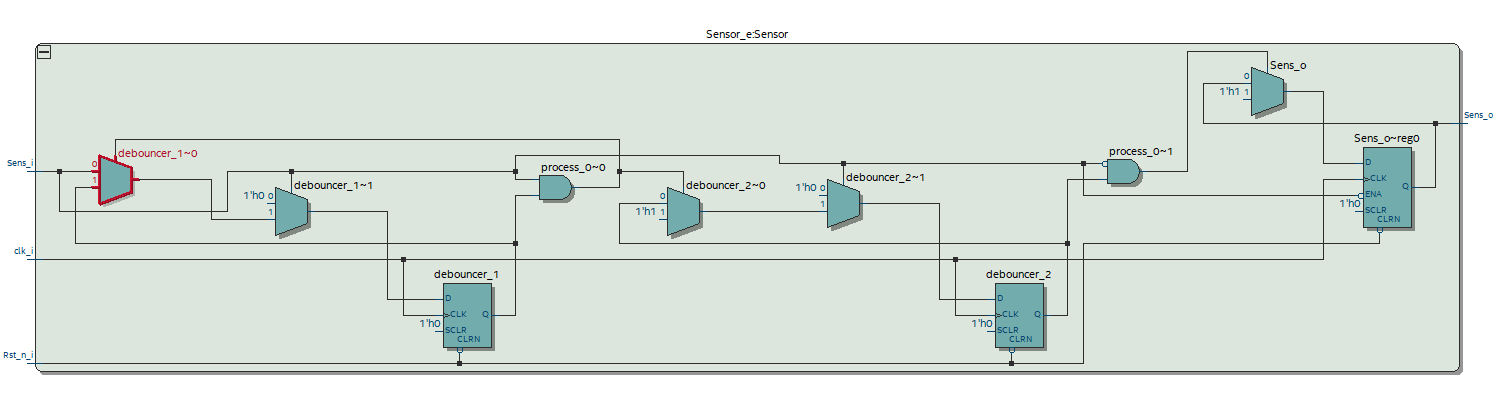
\includegraphics[width=18cm, height=8cm]{db.png}}
	\caption{Debouncer Logic Diagram.}
	\label{fig}
\end{figure}
\vspace{1cm}
\begin{table}[ht!]
	\begin{center}
		\large
		\newcolumntype{P}[1]{>{\centering\arraybackslash}p{#1}}
		\renewcommand{\arraystretch}{1.5}
		\begin{tabular}{ |P{2cm}|P{2cm}|P{2cm}|P{8cm}|}
			\hline
			\rowcolor{gray!50} \textbf{Pin} & \textbf{Direction } & \textbf{Width}  & \textbf{Description} \\
			\hline
			clk\_i & IN & 1 & 12MHz\\
			\hline
			Rst\_n\_i & IN & 1 & Reset, Active Low \\
			\hline
			udb\_i & IN & 1 & Undebounced signal input  \\
			\hline
			db\_o  & OUT & 1 & debounced output signal \\
			\hline
			state1  & Signal & 1 &  \\
			\hline
			state2  & Signal & 1 &  \\
			\hline
		\end{tabular}
	\end{center}
\end{table}


\LARGE
DESCRIPTION \\
\\
\Large
In our system the signal is debounced twice with each rising edge of the CLK. The first time the signal is debounced to check for noise. If after a new rising edge approximately 160 ns the signal is in static state then the debouncer is set to the signal. Then the debouced signal is kept on high until the input signal is goes low. After this the debounced signal is outputed for one clock cycle. This is done in order to make sure that upon each press of the button, even if the button is pushed for more than 160 ns, the system only gets one output cycle. 

\vspace{1.5cm}
\newpage
\section{Finite state machine}
\LARGE
OVERVIEW \\
\\
\Large
FSM consists of limited states. Transitions between different states are done based on current state and an input. FSM are useful when we need to handle a lot of different cases one at a time.  
\vspace{1.5cm}

\begin{figure}[htbp]
	\centerline{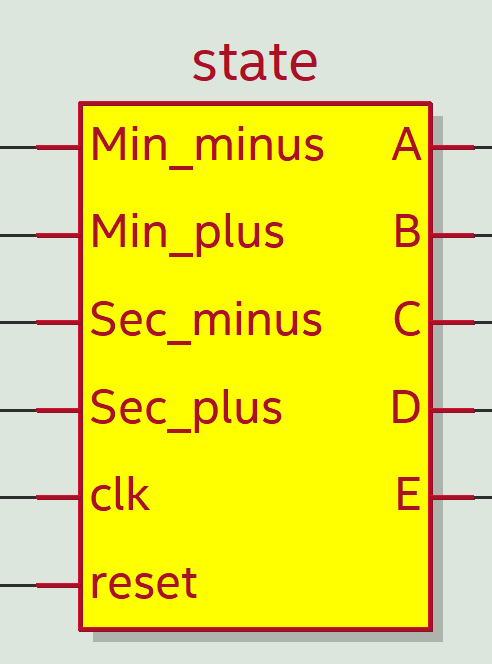
\includegraphics[width=6cm, height=6cm]{fsm1.png}}
	\caption{FSM Top View.}
	\label{fig}
	\vspace{2cm}
	\centerline{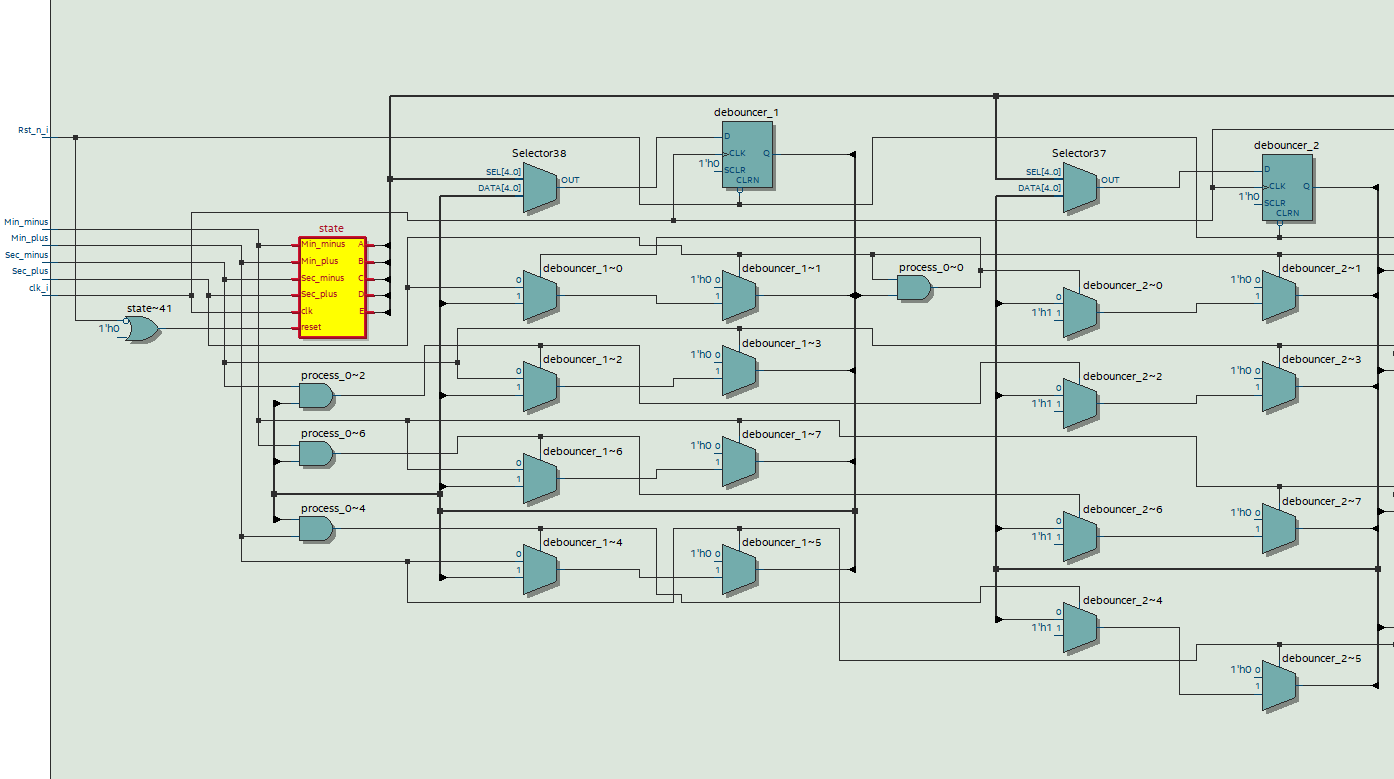
\includegraphics[width=18cm, height=10cm]{fsm2.png}}
	\caption{FSM Logic Diagram.}
	\label{fig}
\end{figure}

\vspace{1cm}

\begin{table}[ht!]
	\begin{center}
		\large
		\newcolumntype{P}[1]{>{\centering\arraybackslash}p{#1}}
		\renewcommand{\arraystretch}{1.5}
		\begin{tabular}{ |P{2cm}|P{2cm}|P{2cm}|P{8cm}|}
			\hline
			\rowcolor{gray!50} \textbf{Pin} & \textbf{Direction } & \textbf{Width}  & \textbf{Description} \\
			\hline
			clk\_i & IN & 1 & 12MHz\\
			\hline
			Rst\_n\_i & IN & 1 & Reset, Active Low \\
			\hline
			state & signal & 1 & \\
			\hline
			FSM\_name & FSM 5 & 1 & \\
			\hline
		\end{tabular}
	\end{center}
\end{table}

\LARGE
DESCRIPTION \\
\\
\Large
Our FSM starts with a initial state which awaits an input signal that will determine the next state to go to. This is done every clock cycle. After we go to one of the other states we will start debouncing the input signal and write to our registers. After the signal debounced and we have an output the FSM goes back to initial state. When in the initial state we check the validity of inputs and continue waiting for other signal to go to different state. The advantage of the FSM in this case is that we are able to deal with one input signal and one process at a time.
\vspace{1.5cm}
\newpage

\section{Uart communication protocol }
\Large
Uart transmission always starts with a start bit which goes from a initial high state to low then the 7 bytes are transmitted (in our case 8N2 transmission)  from the Least significant bit to the highest significant bit. In the end we have two stop bits which go back to high. Every change of the signal happens at a baudrate of 9600 and is synchronized to happen at the middle of each bit.
\vspace{1.5cm}

\begin{figure}[htbp]
	\centerline{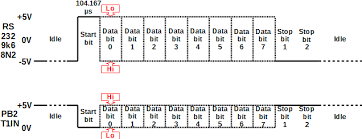
\includegraphics[width=12cm, height=5cm]{uart_com.png}}
	\caption{Uart 8N2 Serial communication.}
	\label{fig}
\end{figure}

\newpage

\chapter{Testbenches}

\Large
\vspace{1cm}
Testbenches are a great tool to test if the complex modules meet all the requirements.
\vspace{1cm}
\begin{itemize}
	\item TopTee\_TB
	\item Alarm\_TB
	\item Counter\_TB
	\item Sensor\_TB
	\item Timer\_TB
	\item UART\_TB
\end{itemize}
\newpage

\chapter{Repository}

\Large
\vspace{1cm}
The Repository contains:
\vspace{1cm}
\begin{itemize}
	\item VHDL Source Code
	\item VHDL Source Code
	\item Documentation
\end{itemize}
\vspace{1cm}
The code can be downloaded via this link: \href{https://github.com/hackvoid/Tea_Brewer}{https://github.com/hackvoid/Tea\_Brewer}\\

\end{document}
